\chapter{Achievement 1}
\label{sec2:ach1}
\section{Problématique}
Jusqu'à présent, les cartes piochées étaient générées aléatoirement dans une sorte de deck virtuel. À partir de l'achievement 1, chaque joueur se voit attribué un deck de 50 cartes en début de partie. Ainsi, lorsqu'un joueur veut piocher une carte pour remplir sa main, il la pioche au sommet de son deck, et lorsqu'il joue une carte, elle est mise dans sa fausse. Quand son deck est vide, les cartes de sa défausse sont mélangées pour reformer un deck.

Il fallait donc intégrer ce nouvel élément dans la dynamique du Base version, en conservant au maximum sa structure et ses fonctions, et notamment en conservant le fichier principal gérant la boucle de jeu tel quel.




\section{Choix d'implémentation}
\subsection{Adaptation des fichiers}
Pour intégrer ce nouvel élément dans la structure précédente, on utilise les avantages de la compilation séparée :
\begin{itemize}
    \item on crée un fichier source \texttt{deck\_ach1.c} contenant la définition de la structure du deck ainsi que les définitions de toutes les fonctions utilisant le deck.
    \item on crée un fichier source \texttt{deck.c} contenant une définition vide de la structure du deck (puisqu'il n'y avait pas de deck dans la Base version) ainsi que les définitions des fonctions de base version équivalentes à celle de \texttt{deck\_ach1.c}, avec des entêtes identiques, quitte à faire des fonctions vides lorsqu'il n'existe pas de telles équivalences.
    \item les fonctions se rapportant au decks ayant ainsi le même prototype dans la Base version et dans l'Achievement, on met les prototypes communs dans le header \texttt{fonctions.h}. Ainsi on compile avec la source \texttt{deck.c} lorsqu'on veut utiliser les fonction pour la Base version, et \texttt{deck\_ach1.c} pour utiliser celles de l'Achievement 1.
\end{itemize} 
Ainsi, comme on peut le voir sur la figure \ref{fig:Orga_Ach1}, la génération du jeu dans les deux versions diffère d'un seule fichier, et l'organisation générale reste proche de celle le la Base version (cf \ref{fig:Base_version_files}).
\begin{figure}
    \centering
    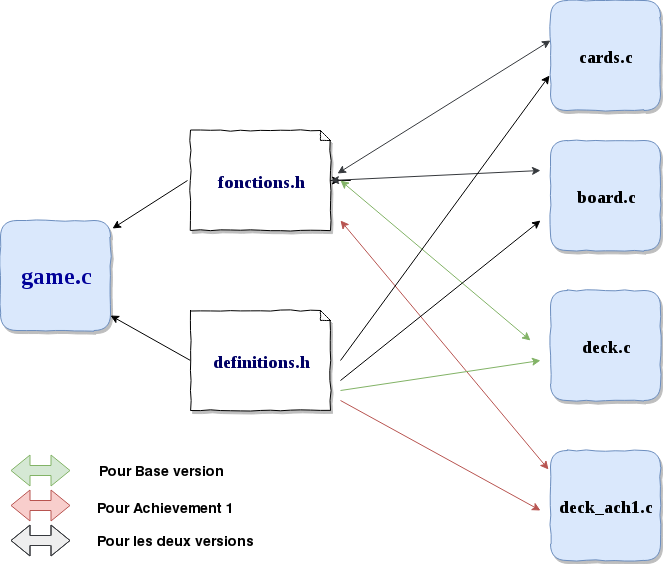
\includegraphics[width=0.8\textwidth]{figures/organisation_Ach1.png}
    \caption{Organisation des fichiers}
    \label{fig:Orga_Ach1}
\end{figure}

Les decks étant tous dans le même fichier source, on y accède seulement grâce à l'adresse de leur zone mémoire, donc on ne les manipule qu'avec des pointeurs. Pour que chaque joueur ait accès à son deck, on a rajouté un champ "deck" qui est un pointeur vers son deck. 

\subsection{Modélisation}

Le deck est modélisé par une file d'identifiants de carte: chaque fois que le joueur pioche une carte, elle est défilée de la file, chaque fois qu'il en défausse une, elle est enfilée à la file.

\begin{figure}[h]
    \centering
    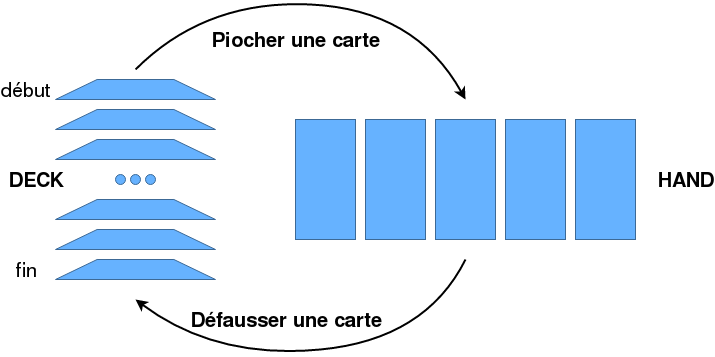
\includegraphics[width=0.8\textwidth]{figures/deck1.png}
    \caption{représentation en file du deck}
    \label{fig:deck_file}
\end{figure}


Pour modéliser cette file en C, on prend un tableau de 50 cartes, parcouru par un indice de début \textbf{top} et un indice de fin \textbf{bottom} (cf \ref{fig:deck_tableau}). Lorsqu'un joueur pioche une carte dans son deck, il récupère l'identifiant de la carte désignée par top puis on incrémente ce dernier; et lorsqu'il se défausse d'une carte après l'avoir jouée, l'identifiant de la carte est enregistrée dans la case désignée par bottom et ce dernier est incrémenté. Les incrémentations se font modulo 50 pour passer de l'indice 49 à 0 et ainsi boucler le tableau sur lui-même. Les cartes allant de top (inclus) à bottom (exclu) sont donc réellement dans le deck, tandis que celles de bottom (inclus) à top (exclu) sont en réalité des places réservées pour les cartes hors du deck (donc dans la main du joueur). Cependant, les identifiants de carte qu'elles contiennent sont quelconques: ce ne sont pas les mêmes que celles dans la main car le joueur ne joue pas ces cartes dans le même ordre qu'il les pioche, d'où l'intérêt d'avoir deux indices.
\begin{figure}[h]
    \centering
    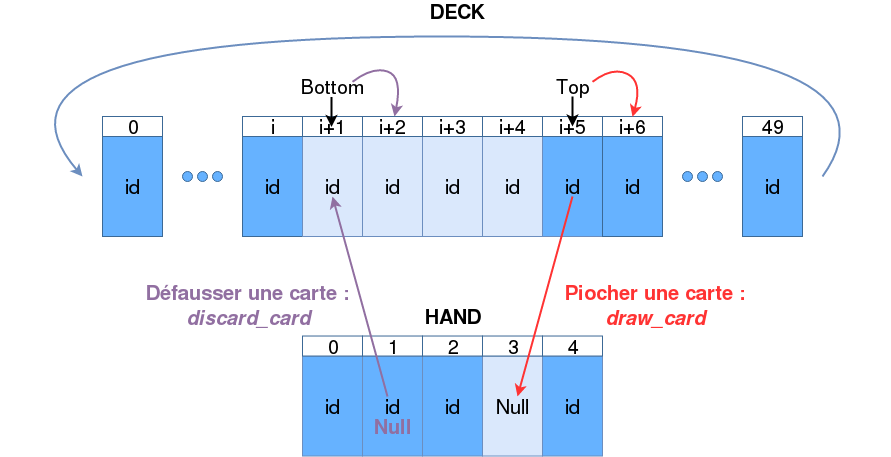
\includegraphics[width=1\textwidth]{figures/deck2.png}
    \caption{représentation avec un tableau du deck}
    \label{fig:deck_tableau}
\end{figure}

Tous les decks des joueurs sont contenus dans un tableau \textbf{decks} statique (sa taille étant fixe, on l'initialise au nombre maximal de joueur autorisé : {\footnotesize MAX\_PLAYERS}). Le champ deck du joueur pointera donc vers la case de ce tableau correspondante.



\subsection{Les fonctions du deck}
\subsubsection{Initialisation des decks }
\label{sec2: initdeck}
L'initialisation des decks se fait en deux temps, la génération de n decks (n étant le nombre de joueur) de 50 cartes prises aléatoirement pour chacun des n joueurs avec \texttt{init\_decks}, et l'attribution de ces decks à leurs propriétaires. L'attribution des decks est fait dans la fonction \texttt{distribute}, qui consiste à copier, pour chaque joueur p, l'adresse du p\up{ième} deck dans son champ deck.

Ces initialisations se font à la fin de l'initialisation du board. pour la Base version, les fonctions équivalentes étaient appelées et ne faisaient rien.\\
\textbf{Complexité :}\\
 L'algorithme d'initialisation \texttt{init\_decks} parcourt donc les l cartes du deck (l étant la longueur d'un deck), pour chacun des n joueurs, et ne fait appel qu'à des fonctions en temps constant, donc sa complexité est en $\theta(l.n)$. Comme la taille des decks est fixée à l=50, on a du $\theta(n)$.\\
La fonction \texttt{distribute} est aussi un parcours du tableau des n joueurs, avec un affectation en temps constant pour chacun, donc il est aussi en  $\theta(n)$.\\
Remarque : la fonction \texttt{init\_board} qui les appelle étant déjà en $\theta(n)$ (cf \ref{sec1: fboard}), sa complexité n'est pas modifiée par l'ajout de ces fonctions.



\subsubsection{fonctions de la dynamique du deck}
Les fonctions \texttt{draw\_card} et \texttt{discard\_card} gèrent l'enfilement et le défilement de la file, selon les règles énoncées plus tôt. On aura toujours bottom $\leq$ top car le joueur l'algorithme du jeu ne permet pas au joueur de jouer plus de carte qu'il n'en a pioché dans son deck, avec égalité quand le deck est plein.\\
\textbf{Complexité :}\\
le fait d'avoir des indices désignant le début et la fin du deck permet de réaliser ces actions en temps constant.\\
Pour \texttt{discard\_card}, il n'y a pas de problème tant que bottom est incrémenté modulo 50.\\
Pour \texttt{draw\_card} en revanche, le problème se pose lorsque top atteint la valeur 50 : le deck est vide, il faut mélanger le deck avant de remettre top à 0. Cependant, il faut faire attention à ne pas prendre les cartes entre bottom (qui vaut normalement 45) et top, qui ne sont pas des cartes dans le deck, car cela modifierait la composition du deck. Le mélange est donc réalisé parmi les cartes de 0 à bottom, et non toutes les cartes du deck.



Le mélange suit l'algorithme suivant : 
\begin{algorithm}
\caption{Algorithme de mélange du deck}
\begin{algorithmic} 
\REQUIRE le deck est réduit à ses indices de 0 à bottom
\FOR{ i indice parcourrant le deck}
\STATE $c \leftarrow $indice aleatoire du deck\\
Echanger les éléments aux indices i et c
\ENDFOR
\end{algorithmic}
\end{algorithm}

Chacune des cartes est échangée au moins une fois avec une cartes prise aléatoirement dans le deck, et en restant entre les indices 0 et bottom, on s'assure bien que seules les cartes présente dans les deck sont prise en compte. 
\\
\textbf{Complexité :}\\
l'algorithme de mélange parcours le deck une fois en faisant des affectations qui se font en temps constant, qui lui même est de taille constante : il est se fait donc en temps constant.

